\section{Our contributions}
\par Our aim is to make full use of exsitent quantum resources for machine learning with big data. In order to handle big data, it is necessary for the speed of training the model to be fast for the data size. Although  variational method is faster than kernel method, it is not sufficient when handling big data. In order to speed up variational method, we want to parallelize variational method with multiple quantum processors.
Furthermore, it is better if there is no need to aggregate given data to the central server, because communication of big data is troublesome (quantum federated learning).
  
\par In this paper, we propose a new distributed coordinate descent algorithm for quantum classification. 

\par Our research has impacts like below:

\begin{enumerate}
\item Our algorithm uses gradient-free optimizer for quantum machine learning, especially for classification. Up until now, algorithms using gradient-free optimizers are mainly focused on optimization problems or chemistry (solving eigenvalue problems for ground state energy computation), not with machine learning. We invent a new algorithm to construct a cost function for quantum classification, which makes it possible to minimize the function gradient-freely.

\item Our algorithm can be parallelized despite using a gradient-free optimizer. Up until now, distributed algorithms were based on gradient-based optimizers\cite{Qi_2022, 9775600}. This is thought to be due to the fact that gradient-free optimizers have not been considered for distributed quantum machine learning algorithms until now because gradient-based optimizers are very associated with classical machine learning. We invent distributed quantum machine learning algorithm using gradient-free optimizers, which are said to converge faster than gradient-based algorithms. This parallelization method makes it possible to do large-scale machine learning using big data.

\item Our algorithm achieves linear-scale speed up in training by the degree of parallelization. This feature is proved theoretically and also indicated by numerical simulations.

\item Our distributed algorithm behaves almost the same as the non-distributed one. Theoretically both behaviors are proved to be completely equal, and numerical simulations support this feature to some extent. Since the recently proposed distributed algorithms use gradient-based optimizers, the results obtained will inevitably change depending on the degree of parallelism. This is the drawback in these distributed algorithms, but we use gradient-free optimizer and that makes it possible to obtain the same result as the non-distributed one.
 \end{enumerate}

\begin{figure}[htb]
    \centering
    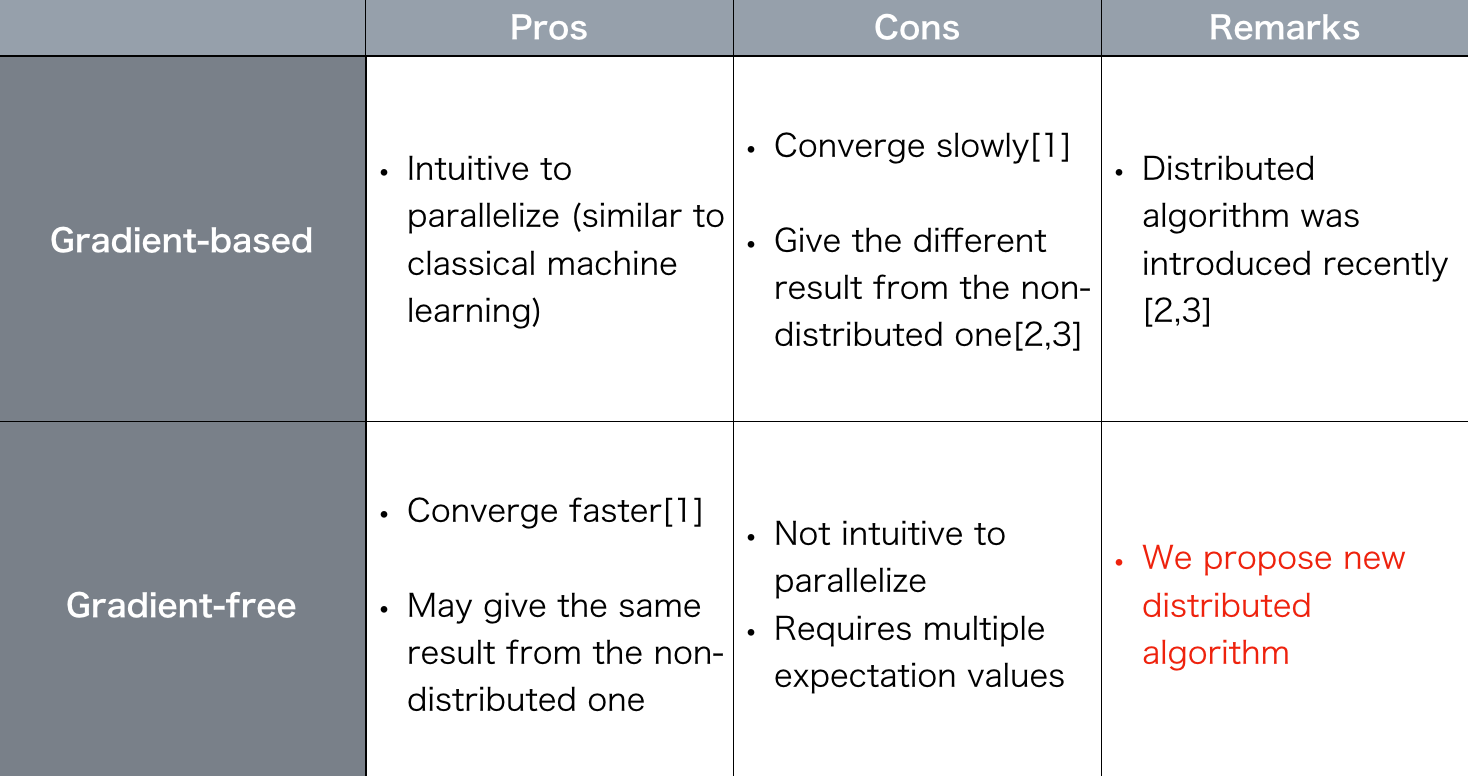
\includegraphics[keepaspectratio, scale=0.5]{introduction/optimizer.png}
    \caption{Our direction compared to the previous researches.}
    \label{fig:optimizer}
\end{figure}